% This file was created by matplotlib2tikz v0.6.18.
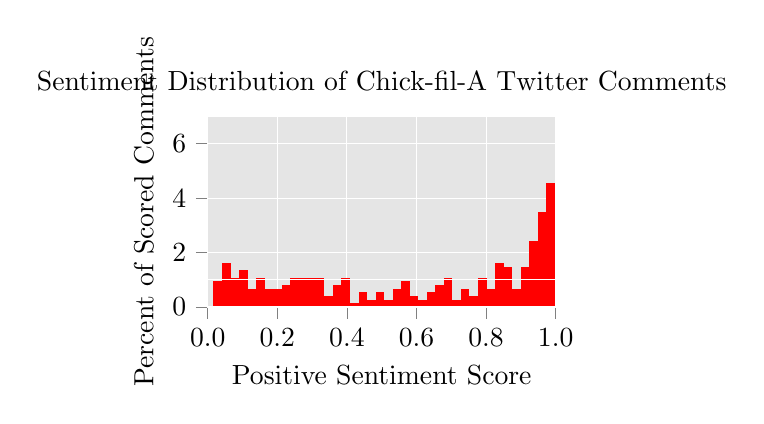
\begin{tikzpicture}

\begin{axis}[
axis background/.style={fill=white!89.80392156862746!black},
axis line style={white},
height=4cm,
tick align=outside,
tick pos=left,
title={Sentiment Distribution of Chick-fil-A Twitter Comments},
width=6cm,
x grid style={white},
xlabel={Positive Sentiment Score},
xmajorgrids,
xmin=0, xmax=1,
xtick={0,0.2,0.4,0.6,0.8,1},
xticklabels={0.0,0.2,0.4,0.6,0.8,1.0},
y grid style={white},
ylabel={Percent of Scored Comments},
ymajorgrids,
ymin=0, ymax=7
]
\draw[fill=red,draw opacity=0] (axis cs:0.0164408497512341,0) rectangle (axis cs:0.0409686155617237,0.941884002379991);
\draw[fill=red,draw opacity=0] (axis cs:0.0409686118364334,0) rectangle (axis cs:0.0654963850975037,1.61465804455914);
\draw[fill=red,draw opacity=0] (axis cs:0.0654963850975037,0) rectangle (axis cs:0.0900241509079933,1.07643885986285);
\draw[fill=red,draw opacity=0] (axis cs:0.0900241583585739,0) rectangle (axis cs:0.114551924169064,1.34554857482856);
\draw[fill=red,draw opacity=0] (axis cs:0.114551916718483,0) rectangle (axis cs:0.139079675078392,0.672774491776985);
\draw[fill=red,draw opacity=0] (axis cs:0.139079660177231,0) rectangle (axis cs:0.163607433438301,1.07643853288272);
\draw[fill=red,draw opacity=0] (axis cs:0.163607448339462,0) rectangle (axis cs:0.188135206699371,0.672774491776985);
\draw[fill=red,draw opacity=0] (axis cs:0.188135206699371,0) rectangle (axis cs:0.212662979960442,0.672774083051698);
\draw[fill=red,draw opacity=0] (axis cs:0.21266296505928,0) rectangle (axis cs:0.237190738320351,0.807328899662038);
\draw[fill=red,draw opacity=0] (axis cs:0.237190753221512,0) rectangle (axis cs:0.261718511581421,1.07643918684318);
\draw[fill=red,draw opacity=0] (axis cs:0.261718511581421,0) rectangle (axis cs:0.28624626994133,1.07643918684318);
\draw[fill=red,draw opacity=0] (axis cs:0.28624626994133,0) rectangle (axis cs:0.310774058103561,1.07643787892305);
\draw[fill=red,draw opacity=0] (axis cs:0.310774028301239,0) rectangle (axis cs:0.335301786661148,1.07643918684318);
\draw[fill=red,draw opacity=0] (axis cs:0.33530181646347,0) rectangle (axis cs:0.35982957482338,0.403664695066191);
\draw[fill=red,draw opacity=0] (axis cs:0.359829545021057,0) rectangle (axis cs:0.384357303380966,0.807329390132381);
\draw[fill=red,draw opacity=0] (axis cs:0.384357333183289,0) rectangle (axis cs:0.40888512134552,1.07643787892305);
\draw[fill=red,draw opacity=0] (axis cs:0.40888512134552,0) rectangle (axis cs:0.433412879705429,0.134554898355397);
\draw[fill=red,draw opacity=0] (axis cs:0.433412849903107,0) rectangle (axis cs:0.457940608263016,0.538219593421588);
\draw[fill=red,draw opacity=0] (axis cs:0.457940638065338,0) rectangle (axis cs:0.482468396425247,0.269109796710794);
\draw[fill=red,draw opacity=0] (axis cs:0.482468366622925,0) rectangle (axis cs:0.506996154785156,0.538219593421588);
\draw[fill=red,draw opacity=0] (axis cs:0.506996154785156,0) rectangle (axis cs:0.531523942947388,0.269109469730763);
\draw[fill=red,draw opacity=0] (axis cs:0.531523942947388,0) rectangle (axis cs:0.556051731109619,0.672773674326908);
\draw[fill=red,draw opacity=0] (axis cs:0.556051731109619,0) rectangle (axis cs:0.580579459667206,0.941885432920666);
\draw[fill=red,draw opacity=0] (axis cs:0.580579459667206,0) rectangle (axis cs:0.605107247829437,0.403664204596145);
\draw[fill=red,draw opacity=0] (axis cs:0.605107247829437,0) rectangle (axis cs:0.629635035991669,0.269109469730763);
\draw[fill=red,draw opacity=0] (axis cs:0.629634976387024,0) rectangle (axis cs:0.654162704944611,0.538220247383238);
\draw[fill=red,draw opacity=0] (axis cs:0.654162764549255,0) rectangle (axis cs:0.678690552711487,0.80732840919229);
\draw[fill=red,draw opacity=0] (axis cs:0.678690552711487,0) rectangle (axis cs:0.703218281269073,1.07644049476648);
\draw[fill=red,draw opacity=0] (axis cs:0.703218281269073,0) rectangle (axis cs:0.727746069431305,0.269109469730763);
\draw[fill=red,draw opacity=0] (axis cs:0.727746069431305,0) rectangle (axis cs:0.752273857593536,0.672773674326908);
\draw[fill=red,draw opacity=0] (axis cs:0.752273797988892,0) rectangle (axis cs:0.776801526546478,0.403665185537428);
\draw[fill=red,draw opacity=0] (axis cs:0.776801586151123,0) rectangle (axis cs:0.801329374313354,1.07643787892305);
\draw[fill=red,draw opacity=0] (axis cs:0.801329374313354,0) rectangle (axis cs:0.825857162475586,0.672773674326908);
\draw[fill=red,draw opacity=0] (axis cs:0.825857162475586,0) rectangle (axis cs:0.850384891033173,1.61466074214971);
\draw[fill=red,draw opacity=0] (axis cs:0.850384891033173,0) rectangle (axis cs:0.874912679195404,1.4801020835192);
\draw[fill=red,draw opacity=0] (axis cs:0.874912619590759,0) rectangle (axis cs:0.899440348148346,0.672775309229047);
\draw[fill=red,draw opacity=0] (axis cs:0.899440407752991,0) rectangle (axis cs:0.923968195915222,1.4801020835192);
\draw[fill=red,draw opacity=0] (axis cs:0.923968195915222,0) rectangle (axis cs:0.948495984077454,2.42198522757687);
\draw[fill=red,draw opacity=0] (axis cs:0.948495984077454,0) rectangle (axis cs:0.97302371263504,3.49843160799105);
\draw[fill=red,draw opacity=0] (axis cs:0.97302371263504,0) rectangle (axis cs:0.997551500797272,4.57486098542298);
\path [draw=white, fill opacity=0] (axis cs:0,0)
--(axis cs:0,7);

\path [draw=white, fill opacity=0] (axis cs:1,0)
--(axis cs:1,7);

\path [draw=white, fill opacity=0] (axis cs:0,0)
--(axis cs:1,0);

\path [draw=white, fill opacity=0] (axis cs:0,1)
--(axis cs:1,1);

\end{axis}

\end{tikzpicture}